\documentclass[sigconf]{acmart}

\usepackage{hyperref}

\usepackage{endfloat}
\renewcommand{\efloatseparator}{\mbox{}} % no new page between figures

\usepackage{booktabs} % For formal tables

\settopmatter{printacmref=false} % Removes citation information below abstract
\renewcommand\footnotetextcopyrightpermission[1]{} % removes footnote with conference information in first column
\pagestyle{plain} % removes running headers

\begin{document}
\title{Big Data Application in Web Search and Text Mining}


\author{Wenxuan Han}
% \orcid{1234-5678-9012}
\affiliation{%
  \institution{Indiana University Bloomingtonn}
  \streetaddress{1150 S Clarizz Blvd}
  \city{Bloomington} 
  \state{Indiana} 
  \postcode{47401-4294}
}
\email{wenxhan@iu.edu}

% The default list of authors is too long for headers}
% \renewcommand{\shortauthors}{B. Trovato et al.}


\begin{abstract}
Because of the rapid development of social media, there are gigantic amount of data generated in every second on the web. And those data could be stored in any forms like text, videos, images or their combinations. The more complicated forms of data, the more space it will take up and will cost more time to read it. Although most of today's personal computers have a very high performance, it is extremely difficult to process and analyze useful text information from those huge amount of unstructured data by using traditional single computer methods without the help of big data tools or text mining techniques. Fortunately, the improvements in big data application are also increasing fast in order to support those difficult works on web search and text mining. In this paper, we first study the data analytic steps in web search, then analyze some of the popular approaches or algorithms (e.g. Hubs, PageRank, etc), and at last, we discuss their applications in this field of big data.
\end{abstract}

\keywords{I523, HID209, Big Data, Social Media, Web Search, Text Mining, PageRank, Hubs}


\maketitle

\section{Introduction}

In recent years, social media has become more and more popular as a new way of communication and knowledge transfer. People could use it to create, share, exchange information and create their own network. Social media usage has been boosted from 2005 to 2015. Users between 18 and 29 ages are the mainly part of social media users \cite{editor01}. Today 90\% of young adults are active on social media. This proportion was 12\% in 2005 \cite{editor02}. And since the development of mobile products, social media has also been offered a better platform for users to share data faster and more convenient. Thus, this proportion could be keep stable or still increase during the next few years.

Nowadays, a growing number of people prefer to express their opinion and feelings through tweeting, sharing images, commenting on social sites \cite{editor01}. Since the amount of such data become extremely large, it is significant to extract and analyze useful information through them by using text analysis methods. Therefore, some applications which based on these information have been developed, such as recommendation system and search engine.

However, as the big data began to appear in the website, there are some problems we must face for web search which include the longer search queries (key words) requirement, support the huge number of searches and multiple languages. And these problems cause the progress of web search and text mining technologies.

Web search is similar to information retrieval (IR) which is used to search for information on the World Wide Web \cite{editor05}. The information may be a mix of web pages, images, and other types of files. Since web search is applying on web, it has a much larger scale than many IR systems. Although web search is a complex technique, it has the capability to understand how to crawl internet to get and update information.

Text mining (also known as knowledge discovery in text database \cite{editor04}) is semi-automatic process of discovering information, meaningful contents, topics, word, relations and patterns from a large amount of text data \cite{editor01}, which is also a branch of data mining. The text data could be extracted by web search at first.

\section{Web Search Technique}

\subsection{Key Fundamental Principles}
DIKW hierarchical model is the most basic model in the information management, information systems and knowledge management disciplines. Thus, it also used behind web search technique. It contains four main components: data, information, knowledge and wisdom. Since we only consider this model in web search area, these four components have the following conception.
\begin{itemize}
\item Data: raw web pages or ``documents viewed as a bag of words''.
\item Information: result of query or ``documents viewed as a collection of insights''.
\item Knowledge: result of processing query results by user.
\item Wisdom: synthesis of many such actions by a set of users.
\end{itemize}

The following fighure shows the hei of DIKW model. We could find that it has a pyramid contructure with wisdom in the top level and data in the bottom level.
\begin{figure}
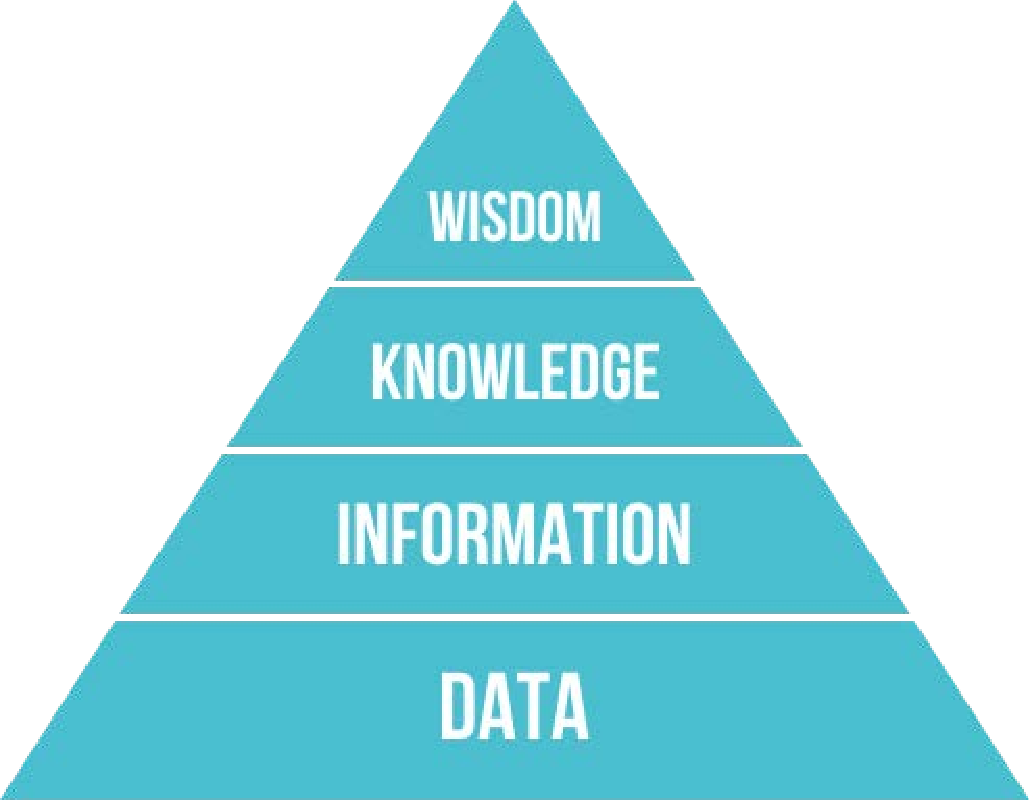
\includegraphics[width=0.30\columnwidth]{images/DIKW_Pyramid}
\caption{DIKW hierarchical model \cite{editor06}.}
\end{figure}

\subsection{Search Engines}
A web search engine is a software system for searching information on the Internet. The search results are generally presented in a line which are often referred to as search engine results pages. And some search engines also haeve the capability to mine data from databases or other open directories. Unlike web directories, which are maintained only by human editors, search engines also maintain web crawling, indexing and searching processes in real-time \cite{editor05}. The following table displays the development of search engines and some searching technologies in recent years.
\begin{table}
\centering
\begin{tabular}{|c|c|} \hline
\textsf{Year} & \textsf{Events} \\ \hline
1990 & First engine ``Archie'' appeared. \\ \hline
1994 & Original Yahoo was human created catalog. \\ \hline
1995-2000 & The classic information retrieval techniques adapted to HTML. \\ \hline 
1998 & Google founded with its link structure by using the PageRank algorithm. \\ \hline
2000-2005 & Add context, spell check, suggestions, multiple sources. \\ \hline
2005- & Add optimization of complete results (e.g. diversity), topic analysis of documents, social search. \\ \hline
\end{tabular}
\caption{Search engines development.}
\end{table}

\subsection{Boolean and Vector Space Models}
Since we already known the basic principles and the application of web search, we now introduce a model that used to define the search technique. Boolean model and vector model are both retrieval model that can be a description of either the computational process or the human process of retrieval. For a retrieval model, it specifies the details of \cite{editor07}: 
\begin{itemize}
\item Document representation.
\item Query representation.
\item Retrieval function (how to find relevant results).
\item Determines a notion of relevance.
\end{itemize}  

In boolean model, keywords are considered to be either present or absent in a
document and to provide equal evidence with respect to information needs. Queries are boolean expressions of keywords, which connected by AND ($\wedge$), OR ($\vee$), and NOT ($\neg$), including the use of brackets to indicate scope \cite{editor07}. Thus, for the output of this model, the result document should be either relevant or not. It could not give partial matches or a ranking. Although this model is easy to understand and offers a clean formalism, it is still complicated for most of web users.

For vector space model, documents and queries are vectors in a high-dimensional space. Assume $t$ distinct terms remain after preprocessing. Each term ($i$) in a document or query ($j$) is given a real valued weight $w_{ij}$. Therefore, both documents and queries are expressed as t-dimensional vectors \cite{editor07}:
\[d_j=(w_{1j},w_{2j},\cdots,w_{tj})\]
There are some patterns to represent term weight. One is the Term Frequency, which assume that important terms have the higher frequency of occurrence in a document. We use the following 
\[tf(t,d)=
  \begin{cases}
    0, & freq(d,t)=0 \\
    1+\log{freq(d,t)}, & \text{otherwise}
  \end{cases}
\]
while $t$ means a typical term, and d means the document.


\subsection{Web Crawling}
\section{Text Mining}
\subsection{lala}

\section{Conclusion}

\begin{acks}

  The authors would like to thank 

\end{acks}

\bibliographystyle{ACM-Reference-Format}
\bibliography{report} 

\end{document}
